\documentclass[11pt,a4paper]{article}
\usepackage{float}
\usepackage{verbatim}
\usepackage{subfig}
\usepackage[T1]{fontenc}
\usepackage[utf8]{inputenc}
\usepackage{geometry}
\usepackage{enumitem}
%\geometry{verbose,lmargin=2cm,rmargin=2cm, bmargin=2cm, tmargin=2cm}
\usepackage{wrapfig}
\usepackage{tikz}
\usetikzlibrary{decorations.markings}
\usepackage{calc}
\usepackage{wrapfig}
\usepackage{graphicx}
\usepackage{amssymb}
\usepackage{amsmath}
\usepackage{esint}
\usepackage{blindtext}
\usepackage{hyperref}
\usepackage{listings}

\hypersetup{
    colorlinks=true,
    linkcolor=blue,
    filecolor=magenta,
    urlcolor=cyan,
}
\usepackage{listings}
\lstset{ %
  backgroundcolor=\color{white},   % choose the background color; you must add \usepackage{color} or \usepackage{xcolor}; should come as last argument
  basicstyle=\footnotesize,        % the size of the fonts that are used for the code
  breakatwhitespace=false,         % sets if automatic breaks should only happen at whitespace
  breaklines=true,                 % sets automatic line breaking
  captionpos=t,                    % sets the caption-position to bottom
  commentstyle=\color{teal},    % comment style
  deletekeywords={...},            % if you want to delete keywords from the given language
  escapeinside={\%*}{*)},          % if you want to add LaTeX within your code
  extendedchars=true,              % lets you use non-ASCII characters; for 8-bits encodings only, does not work with UTF-8
  frame=single,                    % adds a frame around the code
  keepspaces=true,                 % keeps spaces in text, useful for keeping indentation of code (possibly needs columns=flexible)
  keywordstyle=\color{blue},       % keyword style
 % language=Python,                 % the language of the code
  morekeywords={*,...},           % if you want to add more keywords to the set
  numbers=left,                    % where to put the line-numbers; possible values are (none, left, right)
  numbersep=5pt,                   % how far the line-numbers are from the code
  numberstyle=\tiny\color{black}, % the style that is used for the line-numbers
  rulecolor=\color{black},         % if not set, the frame-color may be changed on line-breaks within not-black text (e.g. comments (green here))
  showspaces=false,                % show spaces everywhere adding particular underscores; it overrides 'showstringspaces'
  showstringspaces=false,          % underline spaces within strings only
  showtabs=false,                  % show tabs within strings adding particular underscores
  stepnumber=1,                    % the step between two line-numbers. If it's 1, each line will be numbered
  tabsize=2,                       % sets default tabsize to 2 spaces
  title=\lstname                   % show the filename of files included with \lstinputlisting; also try caption instead of title
}
\begin{document}

\title{Waveoptics\\
\normalsize{FYS2150 Lab Report}}

\author{Nicholas Karlsen}
% \email{nichoka@student.matnat.uio.no}

\date{\today}% It is always \today, today,
%  but any date may be explicitly specified

\maketitle

\begin{abstract}
  Exploring how Laser light behaves when passed through slits and grating of varying kinds and using this behavior to observe the emission lines of Hydrogen, Helium and Cadmium.
\end{abstract}

%\tableofcontents

\section{\label{sect:intro}Introduction}
  This report contains a summary of a lab day in which me and my lab partner performed experiments in which we explored how measurements could be made using the wave-like behavior of light, in particular, diffraction and interference.
  To begin with, we start by looking at the behavior of Laser light diffracted through a wide array of different singular slits, parallel slits and circular slits. After which we measured some of the emission lines of Hydrogen and Helium by the use of diffraction grating and lastly, by the use of an FP-interferometer the split, and slightly shifted emission lines of Cadmium subject to a magnetic field we deduced the Bohr magneton, $\mu_B$, experimentally.

\section{\label{sect:theory}Theory}
  \subsection{Diffraction \& Interference}
    When a monochromatic light wave of wavelength $\lambda$ is passed through a slit of width $a$, the emerging diffraction pattern's measured intensity, $E$, in line, $x$, tangential to the path of the light satisfies the proportionality Eqn. \ref{eqn:single_E}, where $u \equiv x / \lambda R$, $R$ denoting the distance between the slit and the line, $x$.
    \begin{equation}
      E_1(x) \propto a^2 \left( \frac{\sin(\pi a u)}{\pi a u} \right)
      \label{eqn:single_E}
    \end{equation}

    The intensity is at a minimum when $sin(\pi a u) = 0$, which occurs when $au$ is an integer and not zero.

    For two parallel slits with a distance A between, the intensity is instead given by Eqn. \ref{eqn:para_E}, which will have intensity minimum when either $au = n$ for nonzero $n \in \mathbb Z$ or $Au = 2n$ for $n \in \mathbb Z$.

    \begin{equation}
      E_2(x) \propto 4a^2\cos^2(\pi A u) \left( \frac{\sin(\pi a u)}{\pi a u} \right)^2
      \label{eqn:para_E}
    \end{equation}

    This can be generalized for N parallel slits satisfying Eqn. \ref{eqn:N_para}
    \begin{equation}
      E_N(x) \propto a^2 
          \left(
          \frac{\sin (N \pi A u)}{\sin (\pi A u)} \cdot
          \frac{\sin (\pi a u)}{\pi a u}^2
          \right)
          \label{eqn:N_para}
    \end{equation}

    Lastly, for a circular slit the diffraction pattern instead follows a circular symmetry, and its intensity given by Eqn. \ref{eqn:bessel} where $w \equiv \frac{\pi a r}{\lambda R}$, where r denotes the radial distance from the line of light and $J_1$ is the first order bessel function. The first order bessel function is equal to zero for $0, 0.832, 7.016, 10.173$ and $13.324$, which can then be used to predict the expected minima of the intensity distribution.
    \begin{equation}
      E \propto \left( \frac{2 J_1 (w)}{\lambda R} \right)^2
      \label{eqn:bessel}
    \end{equation}


    \subsection{Spectral lines}

      \begin{figure}[H]
        \center 
        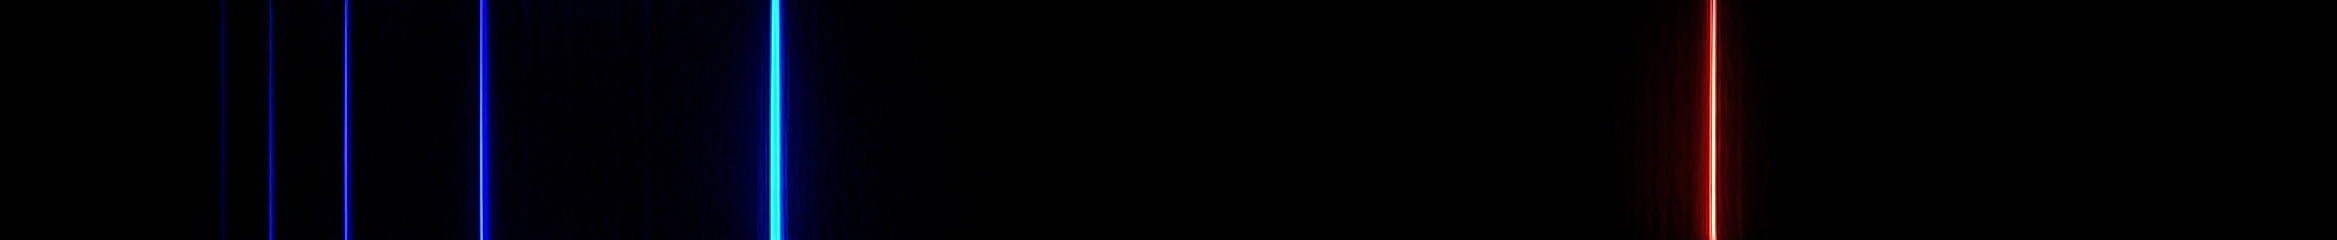
\includegraphics[width=12cm]{scripts/figs/Visible_spectrum_of_hydrogen.jpg}
        \caption{Visible spectrum of hydrogen (Source: \url{https://no.wikipedia.org/wiki/Fil:Visible_spectrum_of_hydrogen.jpg})}
        \label{fig:balmer_lines}
      \end{figure}

      For each chemical element and molecule, there is an associated set of discrete wavelengths  which its emitted light can have. These discrete wavelength are due to internal changes in energy levels, and can be predicted by looking at all the possible changes $\Delta E$ and calculating the wavelength of the photon with this energy by using the Energy-momentum relation \cite{wiki:energy_momentum} and de Broglies equation \cite{wiki:debroglie}.

      Some of the visible lines of hydrogen are referred to as the Balmer series, and is calculated by Eqn. \ref{eqn:balmer} and shown in Fig. \ref{fig:balmer_lines}.
      \begin{equation}
         \lambda_n = \frac{1}{R \left[ \left(\frac{1}{2}\right)^2 - \left(\frac{1}{n}\right)^2 \right]} 
         \label{eqn:balmer}
      \end{equation}

    \subsection{The Zeeman Effect}
      When subject to a uniform magnetic field, $B$, the energy levels of a moluecule are shifted \cite{griffiths}. Resulting in additional, slightly shifted emission lines of wavelengths $\lambda \pm \delta \lambda$. See fig. \ref{fig:zeeman_energy}. with tangential polarization relative to the emission lines for $B=0$.

      \begin{figure}[H]
        \center 
        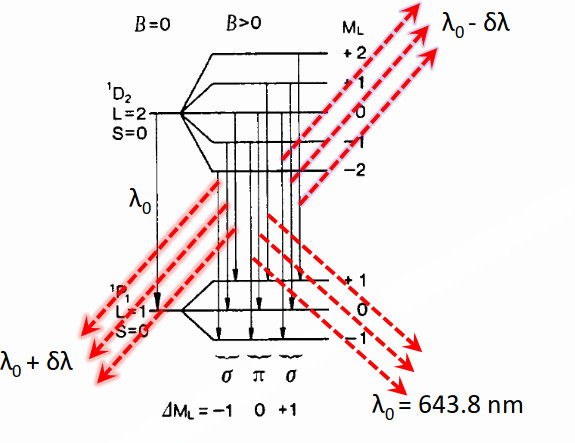
\includegraphics[width=8cm]{scripts/figs/ZEEMAN_ENERGYLEVELS.jpg}
        \caption{Some permitted $\Delta E$ for cadmium, both in and outside of a magnetic field.}
        \label{fig:zeeman_energy}
      \end{figure}


\section{\label{section:experimental}Experimental Procedure} 
    \subsection{Diffraction Grating\label{exp:diffgrat}}
      To investigate the specifications of a selection of slits, and their effect on laser, we used an apparatus as sketched in Fig. \ref{fig:laser}, where a laser lined up with two lenses and a diffraction slit(s) secured on an optical track. Laser passing through is then reflected by a mirror onto a screen in order to effectively increase the distance $R$, in which the laser has passed. This reflection does presumably cause the measurements to deviate slightly from the theoretical model used, but for the purposes of this experiment this deviation is taken to be negligible. 
      Additionally, neither the laser source nor the optical track were fastened to the table and both were easily moved. We took care not to move them, but due to a very limited workspace this may have happened.

      As we swapped between different types slits, the patterns projected onto the screen was recorded by outlining their features on a piece of paper held up to the screen with a pen. Drawing the lines in the "correct" position was not easy to do in a precise manner, and is likely the source of a significant error in our final results across all of the different measurements. Afterwards, distance between the lines was measured using a ruler.

      Also, every time either the mirror or the screen were moved, the distance $R_1$ and/or $R_2$ was measured using a Bosch laser distance measurer.

    \begin{figure}[H]
        \center
        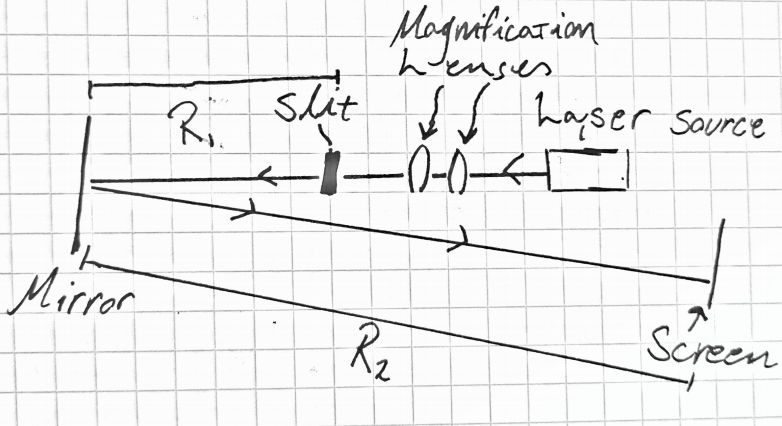
\includegraphics[width=8cm]{scripts/figs/diff_diagram.png}
        \caption{Sketch of apparatus used to measure diffraction lines of a laser}
        \label{fig:laser}
    \end{figure}

    \subsection{Diffraction spectroscopy}

    In order to determine the wavelength of some of the spectral lines in Hydrogen and helium, a spectrometer similar to the one depicted in Fig. \ref{fig:spectrometer} was used. Both the Collimator and the grating were fixed, and whilst the telescope was only fixed radially (relative to the center of the grating). The telescope was connected to a vernier scale, which read its angle $\theta$ relative to the collimator.

    \begin{figure}[H]
        \center
        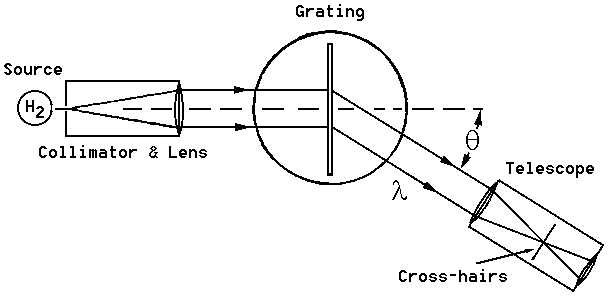
\includegraphics[width=8cm]{scripts/figs/PHY251_H_spectrum_fig1.png}
        \caption{Sketch of spectrometer used to measure angle of diffraction(Source: \url{http://felix.physics.sunysb.edu/~allen/252/PHY251_H_spectrum_fig1.gif})}
        \label{fig:spectrometer}
    \end{figure}

    Light coming from the source is passed through the collimator, hits the grating at a tangent and is diffracted. The visible wavelengths was then be observed through the telescope, and their angle of diffraction recorded by the vernier scale to an accuracy of $10^{-1}\,\textup{deg}$. The diffracted wavelengths were mirrored on both sides, and by taking the difference in their angle on the vernier scale we get $\theta$ satisfying Braggs' law for $n=1$, used to determine the wavelength of the observed spectral line. In addition to recording the angle, we also made note of the color we "think" we saw, which was later used as a way to check the validity of our calculated wavelengths.

    This procedure was performed for both Helium and Hydrogen, for which all clearly visible spectral lines were recorded in succession from the central top (parallel with the collimator) in both the "left" and "right" direction. The angles were recorded in succession from the center in order to ensure that each successive left angle would be in accordance with the corresponding right angle. In addition, we made sure their recorded color matched and that we got the same number of measurements on both sides.

    Lastly, in order for the lines to be visible, the room in which the experiment was performed was kept dark by covering the windows. For the Hydrogen source in particular, additional measures had to be taken by covering the apparatus in a plastic bag whilst finding the spectral lines, in an attempt to filter out make them more visible. This was only partially successful, as the lines were still quite difficult to see clearly.

    \subsection{Zeeman effect\label{sect:zeeman_expt}}
      \begin{figure}[H]
        \center
        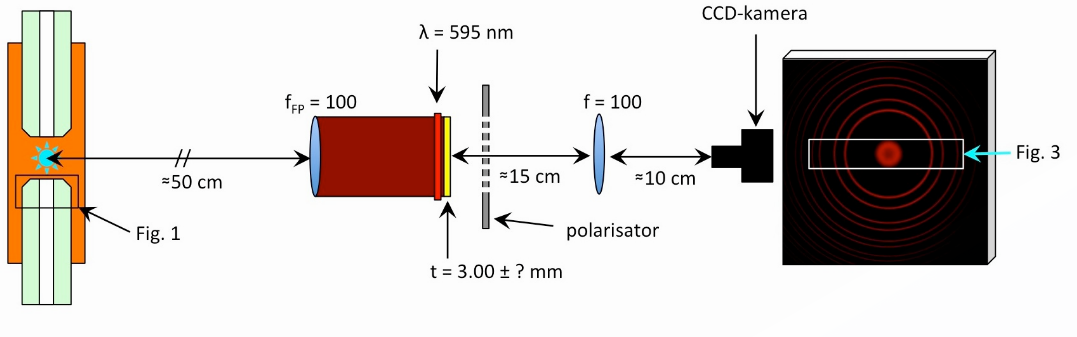
\includegraphics[width=15cm]{scripts/figs/ZEEMAN_EXPERIMENTAL.png}
        \caption{Simplified FP-inferometer}
        \label{FP-inferometer}
      \end{figure}

      An FP-interferometer as was prepared as depicted in Fig. \ref{FP-inferometer}. The source being a cadmium lamp, which light is passed through a focusing lens, filtered by color and polarization, diffracted and focused through another lens before it is recorded by a sensitive camera which is connected to a computer. The exposure, contrast etc is then adjusted to make the diffraction lines as clear as possible.

      Additionally, surrounding the source was an electromagnet connected to a power source. The calibration curve of the electromagnet used is shown in Fig. \ref{fig:cali_curve}. By subjecting the cadmium lamp to a magnetic field, Zeeman splitting can be observed clearly by adjusting the polarization filter such that the original, diffraction pattern are not visible, and the new, "split" lines are fully luminous.

      We saved pictures of these split lines when the current was set to $1, 2, 3$ and $4$ ampere.

      These images were later processed using the script "zeemanread.py" included in appendix \ref{app:scripts}. Which finds the diameter of the first 3 intensity maxima, excluding the central maximum. The script finds the inner and outer edge of each of the rings within 1 pixel, then finds the half-way point between the two as the position of the local intensity maximum. This is then used to deduce the diameter of the rings.

      Whilst this method worked well for $I = 4, 3, 2$ the image for $I=1$ did not have sufficiently separated lines for the script to work, so instead opted to read off the peaks manually by plotting the intensity distribution for a cross section of the image. As shown in Fig. \ref{fig:1A_intensity_dist}.

      From this data, i calculated the value of the Bohr magneton, $\mu_B$ defined in Eqn. \ref{bohrmagneton}, where $d_i$ denotes the diameter of the rings in succession from the center, $hc = 1.98644568\cdot10^{-25}$ and $t$, the thickness of the glass plate in the FP-interferometer in Fig. \ref{FP-inferometer}.

      \begin{equation}
        \mu_b = \frac{hc}{4t} \frac{\sigma}{B},\quad \sigma = \frac{d_2^2 - d_1^2}{d_3^2 - d_1^2}
        \label{bohrmagneton}
      \end{equation}

      I am unable to quantify the uncertainties of this experiment, and will therefore assume that they are negligible. As a result, the only uncertainty i am certain of, is that of $\delta$, which was found to have an uncertainty of $\pm 0.005$ for the rings due resulting from currents, $I=4A, 3A, 2A$ using the formulae for error propagation given in squires \cite{squires_practical_2001}. Based on this error, $\Delta \mu_B$ is then found by Eqn. \ref{eqn:muberror}, where the uncertainties of $hc$, $t$, and $B$ are neglected. The error of $\sigma$ is found by the equations \ref{eqn:sigmaerr}, where $\Delta d =1$. This estimate of the uncertainty results in uncertainties of $\mu_B$ in order of magnitude $10^{-25}$, approximately an order of magnitude larger than the expected value of $\mu_B$.
      \begin{equation}
        \Delta \mu_B = \mu_B \sqrt{\left(\frac{\Delta \delta}{\delta}\right)^2}
        \label{eqn:muberror}
      \end{equation}

      \begin{align}
         \begin{split}
           \Delta d_i^2 &= 2d_i^2\frac{\Delta d_i}{d} = 2d_i\Delta d \\
           \Delta (d_i^2 - d_j^2 ) &= \sqrt{(\Delta d_i^2)^2 + (\Delta d_j^2)^2} = 2\Delta d\sqrt{(d_i)^2 + (d_j)^2} \\
           \Delta\left(\frac{d_i^2 - d_j^2}{d_k^2 - d_j^2}\right) &=
           \left(\frac{d_i^2 - d_j^2}{d_k^2 - d_j^2}\right) 
           \sqrt{ 
            \left(
            \frac{2\Delta d\sqrt{(d_i)^2 + (d_j)^2}}{d_i^2 - d_j^2}
            \right)^2 + 
            \left(
            \frac{2\Delta d\sqrt{(d_k)^2 + (d_j)^2}}{d_k^2 - d_j^2}
            \right)^2 
            }
         \end{split}
         \label{eqn:sigmaerr}
     \end{align} 



      \begin{figure}[H]
        \center
        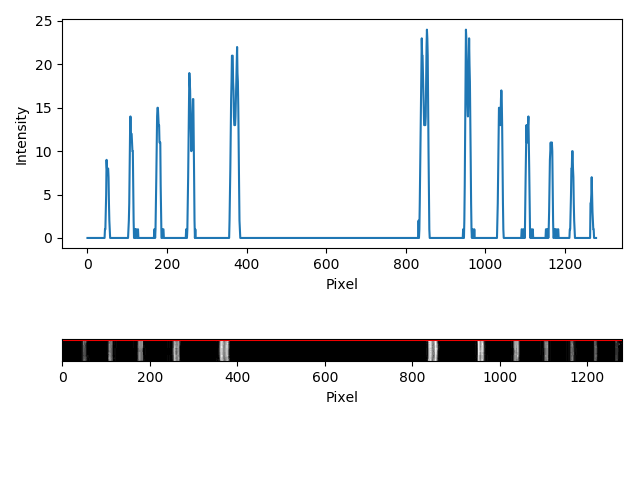
\includegraphics[scale=0.8]{scripts/zeeman_1a_intensity.png}
        \caption{Intensity distribution for cross section of diffraction lines observed for $I=1A$ (top) as well as the associated image (bottom)}
        \label{fig:1A_intensity_dist}
      \end{figure}

      \begin{figure}[H]
        \center
        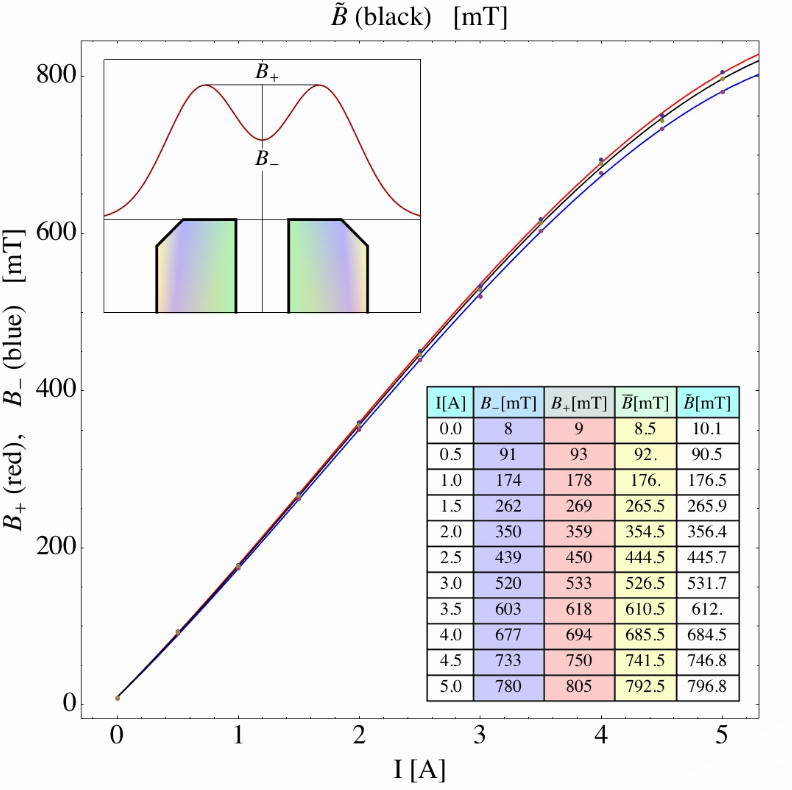
\includegraphics[width=15cm]{scripts/figs/B_calibration_curve.png}
        \caption{Calibration curve for the electromagnet used in the FP-inferometer}
        \label{fig:cali_curve}
      \end{figure}


\section{\label{sect:results}Results}
    \subsection{Diffraction Patterns\label{sect:patterns}}

    In table \ref{tab:singleslit}, i have listed the measured diameter of the primary minimum, the predicted width of the slit based on this along with the width stated by the manufacturer in their data sheet. The length between the diffraction slit and the screen, $R=10.397\pm 0.003m $, was kept constant for the three single slits.

    Similarly in table \ref{tab:circslit}, the calculated diameter based on the inner minimum of the intensity peaks and the length between the diffraction slit and the screen, R.

    Lastly, in table \ref{tab:paraslit} i have listed the observed peaks along with the expected number of visible peaks based on the Width and separation of the slits based on the manufacturers specifications.

    \begin{table}[H]
        \center
        \caption{Single slit}
         \begin{tabular}{l l l}
            Diameter of primary minima [cm] & Calculated Width of Slit [mm] & Stated Width of Slit [mm] \\ \hline
            2.35 & 0.56 & 0.48 \\ 
            4.70 & 0.28 & 0.24 \\
            10.60 & 0.12 & 0.12
         \end{tabular}
         \label{tab:singleslit}
    \end{table}

    \begin{table}[H]
        \center
        \caption{Two parallel slits}
         \begin{tabular}{l l l l}
            Observed No. Peaks & Expected No. Peaks & Width of slits [mm] & Separation of slits [mm] \\ \hline
            9 & 9 & 0.12 & 0.6 \\
            5 & 5 & 0.24 & 0.6 \\
            9 & 11 & 0.24 & 1.2 
         \end{tabular}
         \label{tab:paraslit}
    \end{table}

    \begin{table}[H]
        \center
        \caption{Circular Slit}
         \begin{tabular}{l l l l l l}
            $d_1$ [cm] & $d_2$ [cm] & $d_3$ [cm] & $R$ [m] & Calculated slit diameter [mm] & Stated slit diameter [mm] \\ \hline
            $1.2 \pm 0.1$ & $2.4 \pm 0.1$ & $3.6 \pm 0.1$ & $1.302 \pm  0.003$ & $0.14 \pm 0.01$ & $0.12$ \\ 
            $1.0 \pm 0.1$ & $2.0 \pm 0.1$ & $3.1 \pm 0.1$ & $2.159 \pm  0.003$ & $0.26 \pm 0.01$ & $0.24$ \\ 
            $1.3 \pm 0.1$ & $2.6 \pm 0.1$ & $3.8 \pm 0.1$ & $4.961 \pm  0.003$ & $0.51 \pm 0.01$ & $0.48$ \\ 
         \end{tabular}
         \label{tab:circslit}
    \end{table}


    \subsection{\label{subsect:spectral}Spectral Lines}

    In tables \ref{tab:hydrogen}, \ref{tab:helium} are the wavelengths of the observed emission lines for hydrogen and helium respectively, calculated from $\alpha_v, \alpha_h$ the left and right angular position of the emission lines and $\theta$ denoting the difference between the two.
    
    \begin{table}[H]
        \center
        \caption{Hydrogen Lines}
        \begin{tabular}{ l l l l}
        \input{scripts/dat/hydrogenlines.dat}
        \end{tabular}
        \label{tab:hydrogen}
    \end{table}

    \begin{table}[H]
        \center
        \caption{Helium Lines}
        \begin{tabular}{ l l l l}
            \input{scripts/dat/heliumlines.dat}
        \end{tabular}
        \label{tab:helium}
    \end{table}

    \subsection{\label{subsect:res_Zeeman}Zeeman Effect}

      The pictures taken of the split diffraction lines are shown in Fig.\ref{fig:zeeman_pics} and the associated results computed using the script "zeemanread.py" (see appendix \ref{app:scripts}) are shown in Table \ref{tab:zeeman_table}.

      \begin{figure}[H]
          \center
          \subfloat[][$I = 1\,\textup{A}$]{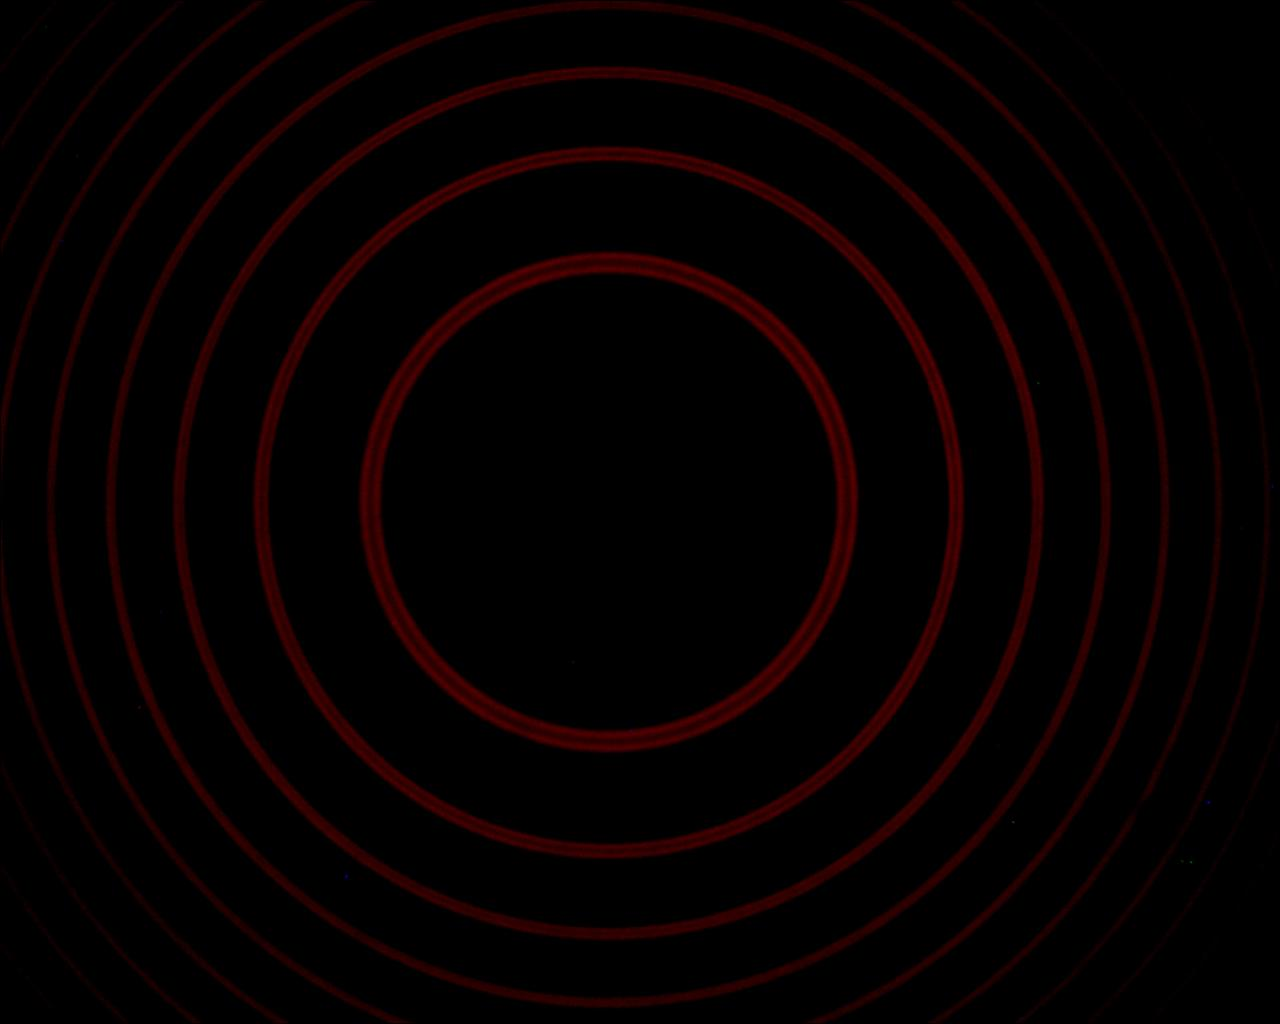
\includegraphics[width=8cm]{scripts/figs/ZEEMAN1A.jpg}\label{fig:zeeman_1A}}
          \subfloat[][$I = 2\,\textup{A}$]{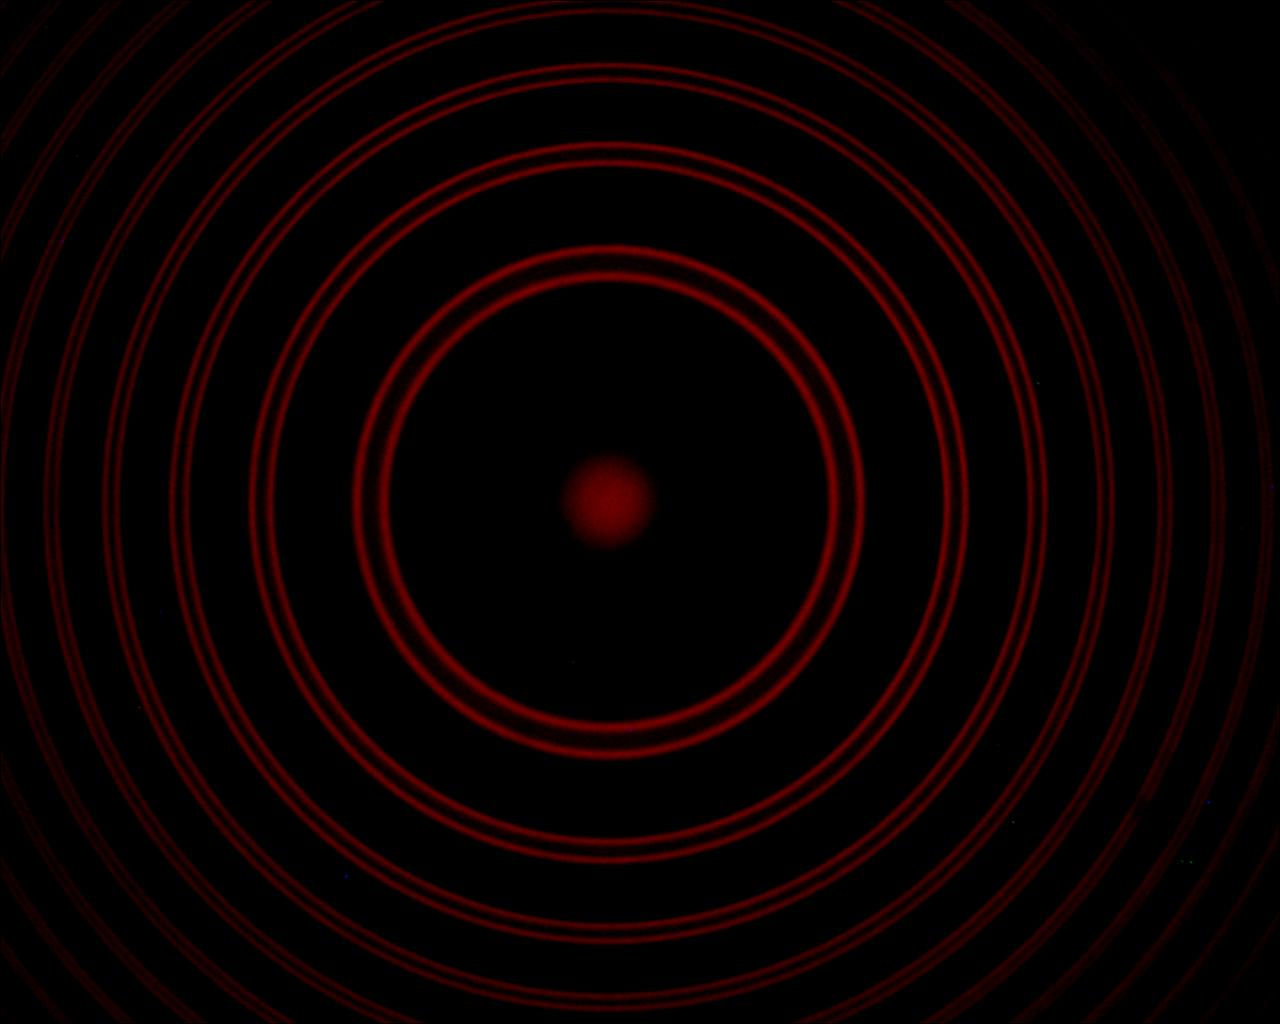
\includegraphics[width=8cm]{scripts/figs/ZEEMAN2A.jpg}\label{fig:zeeman_2A}} \\
          \subfloat[][$I = 3\,\textup{A}$]{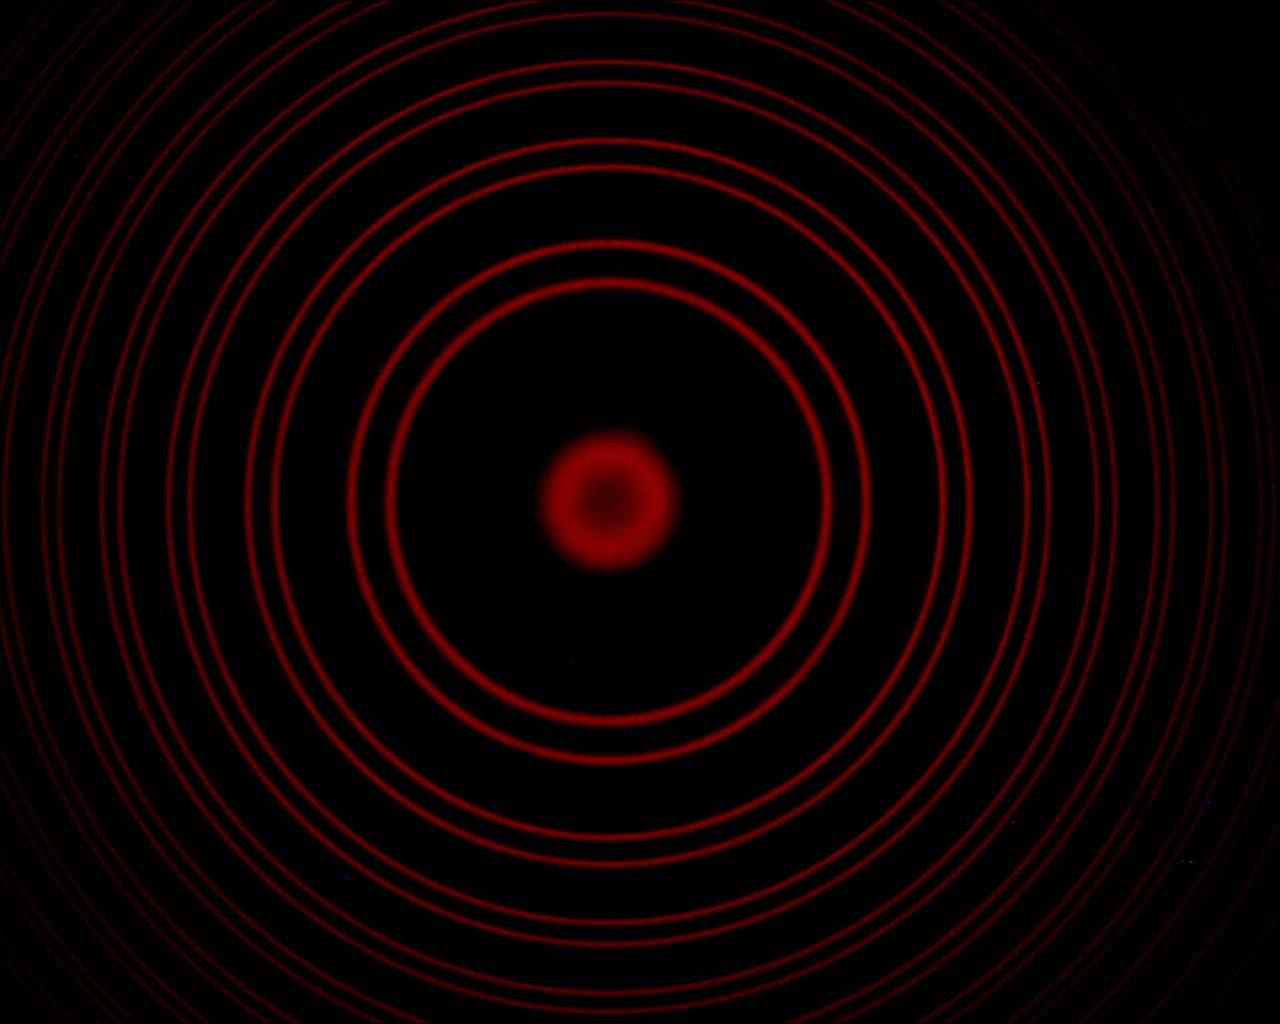
\includegraphics[width=8cm]{scripts/figs/ZEEMAN3A.jpg}\label{fig:zeeman_3A}}
          \subfloat[][$I = 4\,\textup{A}$]{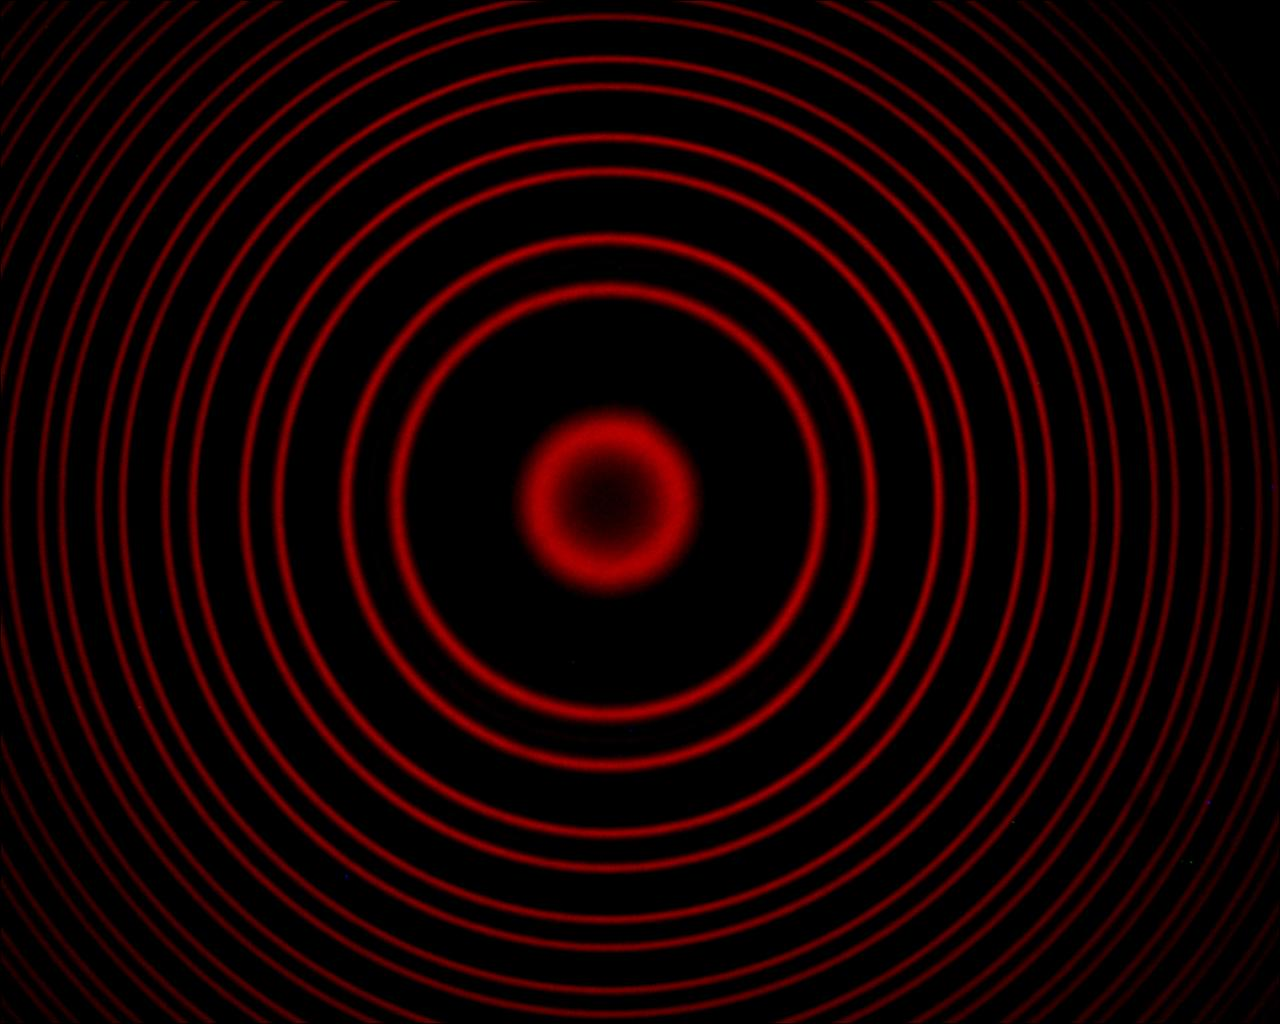
\includegraphics[width=8cm]{scripts/figs/ZEEMAN4A.jpg}\label{fig:zeeman_4A}}
          \caption{Split diffraction lines due to $\sigma$-transitions for different magnitudes of magnetic field}
          \label{fig:zeeman_pics}
      \end{figure}

      \begin{table}[H]
        \center
        \caption{Zeeman results}
        \begin{tabular}{ l  l  l  l  l  r }
          $I$ [A] & $\bar B(I)$ [mT] & $\bar d_1(I)$ [px] & $\bar d_2(I)$ [px] & $\bar d_3(I)$ [px] & $\tilde{\mu_B}$ [$\textup J\,\textup T^{-1}$] \\ \hline

          4 & 685.5 & $423.5 \pm 1$ & $524.5 \pm 1$ & $661.0 \pm 1$ & $8.977\cdot 10^{-24}$ \\
          3 & 526.5 & $437.0 \pm 1$ & $515.0 \pm 1$ & $668.5 \pm 1$ & $9.123\cdot 10^{-24}$ \\ 
          2 & 354.5 & $450.0 \pm 1$ & $503.0 \pm 1$ & $677.5 \pm 1$ & $9.195\cdot 10^{-24}$ \\ 
          1 & 176.0 & $463 \pm 1$ & $489 \pm 1$ & $686 \pm 1$ & $9.086\cdot 10^{-27}$ \\  \hline
            &       &   &     &     &     $\left< \tilde{\mu_B}\right>= 9.095\cdot 10^{-24}$
        \end{tabular}
        \label{tab:zeeman_table}
    \end{table}



\section{\label{sect:discuss}Discussion}
  \subsection{Comparing stated and calculated slit widths based on intensity distribution}
    As mentioned in section \ref{exp:diffgrat}, the experimental setup which was used for the measurements in tables \ref{tab:singleslit}, \ref{tab:circslit} were prone to systematic errors, to put it lightly. As such, it is very likely that the instrumental error due from measuring the distance between the slits and the screen, and the separation of the lines drawn where we "think" the minima were located on the projection screen are essentially negligible compared to the other uncertainties and sources of inaccuracies introduced in the experiment. 

    However, even though the uncertainties are not quite accounted for, the results do seem to correlate with the stated diameter of the slit. One interesting fact to note however, is that every single measurement results in a value greater than (or equal) to the stated width, suggesting that the results may be skewed uniformly in one direction.

  \subsection{Checking the observed emission lines with theory}
    For the balmer series, i expect 4 visible emission lines at 410nm, 434nm, 486nm and 656nm. Looking at our measured data, the emission line $\lambda = 661.25\pm 3.82\,$nm falls reasonably close to an expected emission line, but its range of uncertainty does not quite overlap. As mentioned before, it was noted by my partner that the lines were difficult to see clearly. This likely introduces another source of uncertainty in the measurement which has not been accounted for in the uncertainty calculation. Which along with the already existing instrumental uncertainty makes the two remaining spectral lines highly inaccurate, and matching the two with their theoretical counterpart becomes somewhat difficult due to the significant overlap between the two values and the fact that both of them may be attributed to the expected emission line at 434nm.

    On the other hand, the emission lines from helium were quite distinct, and the observed lines all match up with the expected lines within the uncertainties.

    Therefore, it is obvious that the intensity of the spectrum, and the environment\footnote{As in; the amount of light pollution present} in which the measurements are made pays a significant part in the accuracy of the measurements. Additionally, a significant portion of the "expected" lines did not show up at all, presumably due to a low intensity, which as seen in table \ref{tab:paraslit} can lead to "false" conclusions, where in the last row, observations pointed to 9 intensity peaks, but theory predicted 11. The two remaining peaks were simply too dim to be seen.

  \subsection{Comparison of found $\mu_B$ and reference value}
    CODATA states $\mu_B = 9.274 009 994(57)\times10^{-24}\,J\,T^{-1}$, which means that the mean value of the Bohr magneton, $\left< \tilde{\mu_B}\right>$, deviates $\approx 2\%$ from the reference value, not accounting for uncertainties. Seeing as all 4 measurements fall close to this individually, i suspect my estimation for the error $\Delta \delta$ as discussed in \ref{sect:zeeman_expt} may be a gross over-estimation. Further, without any significant insight into the precision of the FP-interferometer, it is difficult to assert whether the deviation between the CODATA value and the measured result can be attributed to experimental uncertainties, or errors in the post-processing of the results.

\section{\label{sect:conclusion}Conclusion}
  When performing experiments of this nature, quantifying the potential errors that may occur outside of the instrumental uncertainties seems quite a difficult task. Regardless, the deviation between what is expected and what is measured using these techniques seems to only deviate by a few percent, even when the methodology is seemingly prone to errors. And ultimately, considering the scales at which these macroscopic experiments measure, it is notable that the measurements "only" seems to deviate by a few percent of what is expected.

\bibliographystyle{plain}
\bibliography{references.bib}

%%%%%%%%%%%%%%%%%%%%%%%%
%%% END OF MAIN BODY %%%
%%%%%%%%%%%%%%%%%%%%%%%%
\newpage
\appendix
\section{Scripts\label{app:scripts}}
\lstinputlisting[language=python]{scripts/zeemanread.py}

\end{document}